\begin{center}
\large Experimento: \textbf{Amplificador somador inversor}
\end{center}


\section{Introdução}

O presente relatório visa detalhar o experimento laboratorial realizado na disciplina laboratório de circuitos eletrônicos no dia 17 de setembro de 2019 sobre amplificador somador inversor utilizando amplificadores operacionais, mais especificamente os do circuito integrado LM741.

Esses amplificadores somadores inversores possuem as mais diversas aplicações, pois permitem que dois ou mais sinais sejam amplificados com diversos ganhos e que sejam somados e por fim invertidos. 

A prática tem o objetivo de comprovar na prática os efeitos na saída do amplificador com diversas configurações de entradas. Bem como avaliar o ganho para cada uma das entradas. O circuito do amplificador a ser montado etá disposto na figura \ref{ckt:1}, sendo $R_1 = 10 \kilo \ohm$, $R_2 = 4.7 \kilo \ohm$, $R_3 = 10 \kilo \ohm$ e $R_4 = 2.2 \kilo \ohm$.

\begin{figure}[H]
\begin{center}
\begin{tikzpicture} [ american, ]
    \draw (0,0) node[op amp] (opamp) {}
    (opamp.+) -- (-2,-0.5) %node[left] {$V_{in}$}
    (opamp.-) -- (-2.5,0.5)
    (opamp.out) --  (2,0) node[right] {$V_o$}
    (opamp.up) --++(0,0.25) node[vcc]{15\,\textnormal{V}}
    (opamp.down) --++(0,-0.25) node[vee]{-15\,\textnormal{V}}
    (-2.5,0.5) to[short,-] (-2.5,2.5)
    (1.5,0) to[short,*-] (1.5,2.5)
    (-2.5,2.5) to[R,l=$R_3$] (1.5,2.5)
    (-2,-3) node[ground]{} to[R, l=$R_4$] (-2,-0.5)
    (-5,0.5) node[left] {$V_1$} to[R, l=$R_1$, *-*] (-2.5,0.5)
    (-5,-1) node[left] {$V_2$} to[R,l=$R_2$,*-] (-2.5,-1)
    (-2.5,0.5) -- (-2.5,-1)
    ;
\end{tikzpicture}

\end{center}
\caption{Amplificador somador inversor.}
\label{ckt:1} 
\end{figure}


Como forma de auxiliar na compreensão da prática, foi utilizado um segundo circuito, cuja saída servirá como umas das entradas do amplificador. Esse circuito está disposto na figura \ref{ckt:2}, com $V_{CC} = 15V$ e utiliza-se de um divisor de tensão com um potenciômetro para a criação de um nível DC desejado, logo após passando por um \textit{buffer} de tensão.

\begin{figure}[H]
\begin{center}
\begin{tikzpicture} [ american, ]
    %shorts
    \draw (0,0) node[op amp] (opamp) {}
    (opamp.+) -- (-2.5,-0.5) %node[left] {$V_{in}$}
    (opamp.-) -- (-1.5,0.5)
    (opamp.out) --  (2,0) node[right] {$V_x$}
    (opamp.up) --++(0,0.25) node[vcc]{15\,\textnormal{V}}
    (opamp.down) --++(0,-0.25) node[vee]{-15\,\textnormal{V}}
    (1.5,0) to[short, *-] (1.5,2)
    (1.5,2) -- (-1.5,2) -- (-1.5,0.5)
    (-3,1.25) node[left] {$+V_{CC}$} to[pR, l_=$100k \ohm$, *-*] node[left] {$-V_{CC}$} (-3,-2.25)
    ;
\end{tikzpicture}
\end{center}
\caption{Divisor de tensão com \textit{buffer}.}
\label{ckt:2} 
\end{figure}

Inicialmente calculou-se o ganho de tensão correspondente a cada uma das entradas do amplificador somador inversor. Logo após fora montado e verificado o circuito da figura \ref{ckt:2}, avaliando o nível DC na saída. Por fim, o amplificador foi alimentado em ambas as entradas, com a primeira sendo alimentada por uma senoide e a outra com o nível DC obtido do circuito \ref{ckt:2}. Assim, permitiu-se constatar os efeitos que cada uma das entradas possuem na saída do circuito \ref{ckt:1}.

O osciloscópio digital foi utilizado para medir as formas de onda na entrada e na saída do amplificador somador inversor, como forma de comparar os valores e comprovar os resultados teóricos.

\section{Análise Teórica}



\subsection{Amplificador Somador Inversor}

O circuito amplificador somador inversor é um dos mais utilizados circuitos usando o amplificador operacional como base, devido a possibilidade de somar sinais analógicos, sendo que a saída é proporcional (com um fator de ganho constante) ao negativo da soma das entradas.
Para a análise teórica devemos relembrar de forma rápida como calcular os parâmetros de saída do amplificador somador inversor.


\begin{figure}[H]
\begin{center}
\begin{tikzpicture} [ american, ]
    \draw (0,0) node[op amp] (opamp) {}
    (opamp.+) -- (-1.5,-0.5) %node[left] {$V_{in}$}
    (opamp.-) -- (-2.5,0.5)
    (opamp.out) --  (2,0) node[right] {$V_o$}

    (-2.5,0.5) to[short,-] (-2.5,2)
    (1.5,0) to[short,*-] (1.5,2.5)
    (-1.5,0.5) to[short,*-] (-1.5,2.5)
    (-1.5,2.5) to[R,l=$R_f$, i=$I_f$, v=$V_{Rf}$,] (1.5,2.5)
    (-1.5,-0.5) node[ground]{}
    (-5,2) node[left] {$V_1$} to[R,l=$R_1$, i=$I_1$, *-] (-2.5,2)
    (-5,0.5) node[left] {$V_2$} to[R, l=$R_2$, i=$I_2$,*-*] (-2.5,0.5)
    (-5,-1) node[left] {$V_n$} to[R,l=$R_n$, i=$I_n$,*-] (-2.5,-1)
    (-2.5,0.5) -- (-2.5,-1)
    (-4.7,-0.05) to[short,*-] (-4.7,-0.05)
    (-4.7,-0.25) to[short,*-] (-4.7,-0.25)
    (-4.7,-0.45) to[short,*-] (-4.7,-0.45)
    ;
\end{tikzpicture}

\end{center}
\caption{Amplificador somador inversor genérico de n entradas.}
\label{ckt:3} 
\end{figure}


Primeiramente como há uma malha de realimentação negativa no circuito da figura acima, logo:

\begin{center}
    $V^- = V^+ = 0 $
\end{center}

Dessa forma,


\begin{center}
    $I_k = \frac{V_k}{R_k} \hspace{5}  \forall \hspace{5} k \in [1;n]$
\end{center}

Sabemos que $I^+ = I^- = 0$.

Todas as correntes $I_k$ se juntam vão para $R_f$ e criam $I_f$:

\begin{center}
    $I_f = \sum\limits_{k = 1}^{n}I_k $
\end{center}

Logo a corrente $I_f$ vai toda para $R_f$, e de imediato sua tensão será:

\begin{center}
    $V_{Rf} = R_f \times I_f = R_f \times \sum\limits_{k = 1}^{n}I_k  $
\end{center}


\begin{center}
    $V_{Rf} = R_f \times (I_1 + I_2 + I_3 +...+I_n) = \left (\frac{R_f}{R_1} \times V_1 + \frac{R_f}{R_2} \times V_2 + \frac{R_f}{R_3} \times V_3 +...+ \frac{R_f}{R_n} \times V_n \right)$
\end{center}

Como 

\begin{center}
$V_o = V^- - V_{Rf} = 0 - V_{Rf} =-V_{Rf}  $
\end{center}


Portanto,

\begin{center}
    $V_{o} = - \left(\frac{R_f}{R_1} \times V_1 + \frac{R_f}{R_2} \times V_2 + \frac{R_f}{R_3} \times V_3 +...+ \frac{R_f}{R_n} \times V_n \right)$
\end{center}

Para o circuito somador inversor da figura \ref{ckt:1}, temos apenas duas entradas, logo:

\begin{center}
    $V_{o} = - \left(\frac{R_f}{R_1} \times V_1 + \frac{R_f}{R_2} \times V_2 \right)$
\end{center}

A análise do circuito da figura \ref{ckt:2}, é um seguidor de tensão unitário que é um circuito que fornece ganho unitário sem inversão de fase, logo:

\begin{center}
    $V_{x} = V^+$
\end{center}

\subsection{Resultados Teóricos}

Primeiramente utilizando o circuito da figura \ref{ckt:1}, devemos calcular $A_v$ para ambas as entradas individuais. Ou seja, 

\begin{itemize}
    \item Para $V_1 = sen(2\pi.1000t)$ e $V_2 = 0$:
    \begin{center}
        $A_{v1} = - \frac{10 \times 10^3}{10 \times 10^3} = - 1 $ V/V
    \end{center}
    
    Portanto o sinal de entrada será apenas invertido na saída.
    
    \begin{center}
        $V_{o} = -sen(2\pi.1000t) $ V
    \end{center}
    
    \item Para $V_1 = 0 $ e $V_2 = sen(2\pi.1000t)$:
    
    \begin{center}
        $A_{v2} = - \frac{10 \times 10^3}{4.7 \times 10^3} = - 2.127 $ V/V
    \end{center}
    
    Portanto o sinal de saída será aproximadamente o dobro de sinal de entrada.
    
    \begin{center}
        $V_{o} = -2.127 \times sen(2\pi.1000t) $ V
    \end{center}
    
\end{itemize}


Foi ajustado o circuito da figura \ref{ckt:2} para se ter $ V_x = 1V$ e $V_x = 2V$ no nível DC do sistema, para dois sistemas diferentes. Com isso foi possível analisar o amplificador somador com as duas entradas ativas para ambos os sistemas. $V_1$ sendo a senóide e V2 sendo o nível DC. Logo obtemos na saída.

\begin{itemize}
    \item Para $V_1 = sen(2\pi.1000t)$ e $V_2 = 1V$:
    \begin{center}
        $V_{o} = - \left(\frac{10 \times 10^3}{10 \times 10^3} \times  sen(2\pi.1000t) + \frac{10 \times 10^3}{4.7 \times 10^3} \times 1 \right)$
    \end{center}
     \begin{center}
        $V_{o} = - 2.127 - sen(2\pi.1000t) $ V
    \end{center}
    
    
    \item Para $V_1 = sen(2\pi.1000t) $ e $V_2 = 2V$:
    
    \begin{center}
        $V_{o} = - \left(\frac{10 \times 10^3}{10 \times 10^3} \times  sen(2\pi.1000t) + \frac{10 \times 10^3}{4.7 \times 10^3} \times 2 \right)$
    \end{center}
     \begin{center}
        $V_{o} = - 4.255 - sen(2\pi.1000t) $ V
    \end{center}
\end{itemize}



\section{Resultados e discussão}

Para encontrar todos os resultados necessários para comprovar a teoria, a prática foi dividida em algumas etapas, sendo elas:

\begin{itemize}
    \item Medição dos ganhos de cada uma das entradas;
    \item Montar e verificar a saída do cicuito da figura \ref{ckt:2};
    \item Aplicar nas entradas do circuito da figura \ref{ckt:1} uma senoide e o nível DC varíavel oriundo da saída do circuito \ref{ckt:2};
\end{itemize}

Para a medição do ganho devido a entrada 1, a entrada 2 foi aterrada ($V_2=0$) e a entrada 1 ($V_1$) foi alimentada com uma senoide de 1 V de pico e 1kHz de frequência. Assim, obteu-se as formas de onda da figura \ref{p2-out}. Considerando o canal 1 (cor clara) como a entrada e o canal 2 (cor escura) como a saída, observa-se pouca alteração na amplitude da saída, porém com a inversão de fase devido ao amplificador inversor. Dessa forma o ganho de tensão devido a entrada 1 obervada na figura \ref{p2-out} será:

\begin{center}
    $A_{v1} = -\frac{2.02}{2.02} = -1 V/V$
\end{center}

\begin{figure}[H] 
\includegraphics[scale=2.5]{imagens/p2-output.jpg} 
\centering
\caption{Saída do circuito amplificador, com $V_2=0$ e $V_1=1.01 sen(2\pi1000t)$}
\label{p2-out} 
\end{figure} 

De forma semelhante foi medido o ganho devido a entrada 2. Sendo que a entrada 1 foi aterrada ($V_1=0$) e a entrada 2 ($V_2$) foi alimentada com uma senoide de 1 V de pico e 1kHz de frequência. Assim, obteu-se as formas de onda da figura \ref{p3-out}. Considerando o canal 1 (cor clara) como a entrada e o canal 2 (cor escura) como a saída, observa-se uma alteração significante na amplitude do sinal de saída e a sua inversão de fase. Dessa forma o ganho de tensão devido a entrada 2 obervada na figura \ref{p3-out} será:


\begin{center}
    $A_{v1} = -\frac{4.35}{2.02} = -2.153 V/V$
\end{center}

\begin{figure}[H] 
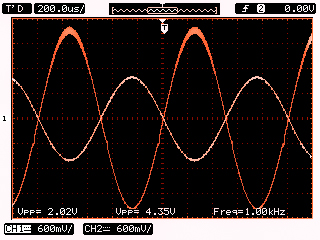
\includegraphics[scale=2.5]{imagens/p3-output.jpg} 
\centering
\caption{Saída do circuito amplificador, com $V_1=0$ e $V_2=1.01 sen(2\pi1000t)$}
\label{p3-out} 
\end{figure} 

A tabela \ref{tab:1} compara os valores teóricos e práticos de cada uma das saídas, mostrando uma ótima correspondência entre os valores, com um erro de cerca de 1,2\% para a saída 2 e erro nulo para a saída 1.

\begin{table}[H]
\centering
\begin{tabular}{c|c|c|}
\hline
\multicolumn{1}{|c|}{} & {$A_{v1}$} &  {$A_{v2}$}\\ \hline
\multicolumn{1}{|c|}{Ganho teórico} & {-1 V/V} &  {-2.127 V/V}\\ \hline
\multicolumn{1}{|c|}{Ganho prático} & {-1 V/V} &  {-2.153 V/V}\\ \hline
\end{tabular}
\caption{Comparação dos ganhos de tensão devido a cada uma das entradas.}
\label{tab:1}
\end{table}

Finalizada a primeira etapa, permite-se que, em seguida, o circuito da figura \ref{ckt:2} fosse avaliado. De acordo com a forma de onda da figura \ref{p4-out} observa-se a saída do circuito ajustada em 1V, porém com a capacidade de variar na faixa de $-14 V \leq V_x \leq 14.4 V$, como verificado na prática ao ajustar o potenciômetro. 

%Uma hipótese para a limitação da tensão pode ter sido devido a ruídos no potenciômetro, pois também se constatou que ao aumentar a tensão na saída desse circuito, o ruído no sinal DC também aumentava.


\begin{figure}[H] 
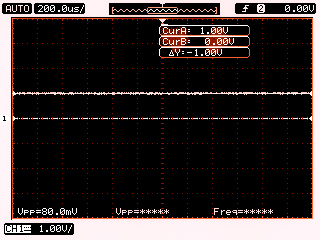
\includegraphics[scale=2.5]{imagens/p4-output.jpg} 
\centering
\caption{Saída do divisor de tensão}
\label{p4-out} 
\end{figure} 

Em seguida fora testada a etapa final, com o amplificador somador inversor funcionando com ambas as entradas como proposto inicialmente. O potenciômetro foi ajustado em dois casos para obter um nível DC de 1V e 2V em $V_x$. Dessa forma, foram geradas as formas de onda da figura \ref{p5-1} para o primeiro caso e as formas de onda da figura \ref{p5-2} para o segundo caso.

\begin{figure}[H] 
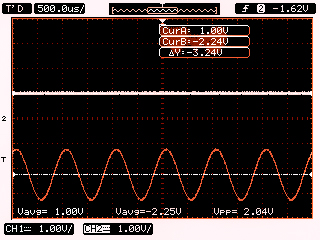
\includegraphics[scale=2.5]{imagens/p5-v2-1V.jpg} 
\centering
\caption{Saída do amplificador somar inversor para $V_2=1V$.}
\label{p5-1} 
\end{figure} 

\begin{figure}[H] 
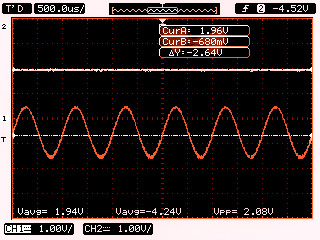
\includegraphics[scale=2.5]{imagens/p5-v2-2V.jpg} 
\centering
\caption{Saída do amplificador somar inversor para $V_2=2V$.}
\label{p5-2} 
\end{figure} 

Observa-se que para a entrada $V_2= 1V$ na figura \ref{p5-1} o sinal amplificado foi deslocado de $A_{v2}V_2$, ficando centrado em cerca de -2.25 V, cujo valor previsto na teoria foi -2.127 V. O sinal senoidal, como foi inserido na entrada de ganho unitário, teve apenas sua fase atrasada de 180°, porém com a mesma amplitude.

Na figura \ref{p5-2} com a entrada $V_2= 2V$, o sinal foi deslocado mais ainda considerando a contribuição de $A_{v2}V_2$ na saída do amplificador somador inversor, contribuindo para que o sinal senoidal, que foi apenas defasado de 180° e ganho unitário, ficasse centrado em -4.24 V, cujo valor previsto na teoria foi -4.255 V.

Esses resultados corroboram com os encontrados durante a análise teórica, permitindo validar os resultados encontrados na prática.

\section{Conclusões}

Nesta prática foi estudado o circuito amplificador somador inversor, foi possível realizar sua montagem e fazer a análise dos parâmetros de saída do sinal do circuito proposto, primeiramente foi analisado às entradas separadamente de cada um dos circuitos, tanto para o amplificador somador inversor tanto para o seguidor tensão unitária, com divisor de tensão (com o potenciômetro). Após isso, foi analisado como a saída se comportava para ambas entradas com valores definidos de tensão, um com valor alternado e com valor contínuo. Portanto, percebeu que os parâmetros medidos em prática aproximaram-se bastante com os valores calculados e com isso se constatou que de fato a saída do amplificador somador inversor corresponde a soma dos sinais de entradas invertidos, como era esperado teoricamente. 

\newpage

\section{Anexos}

\begin{figure}[H] 
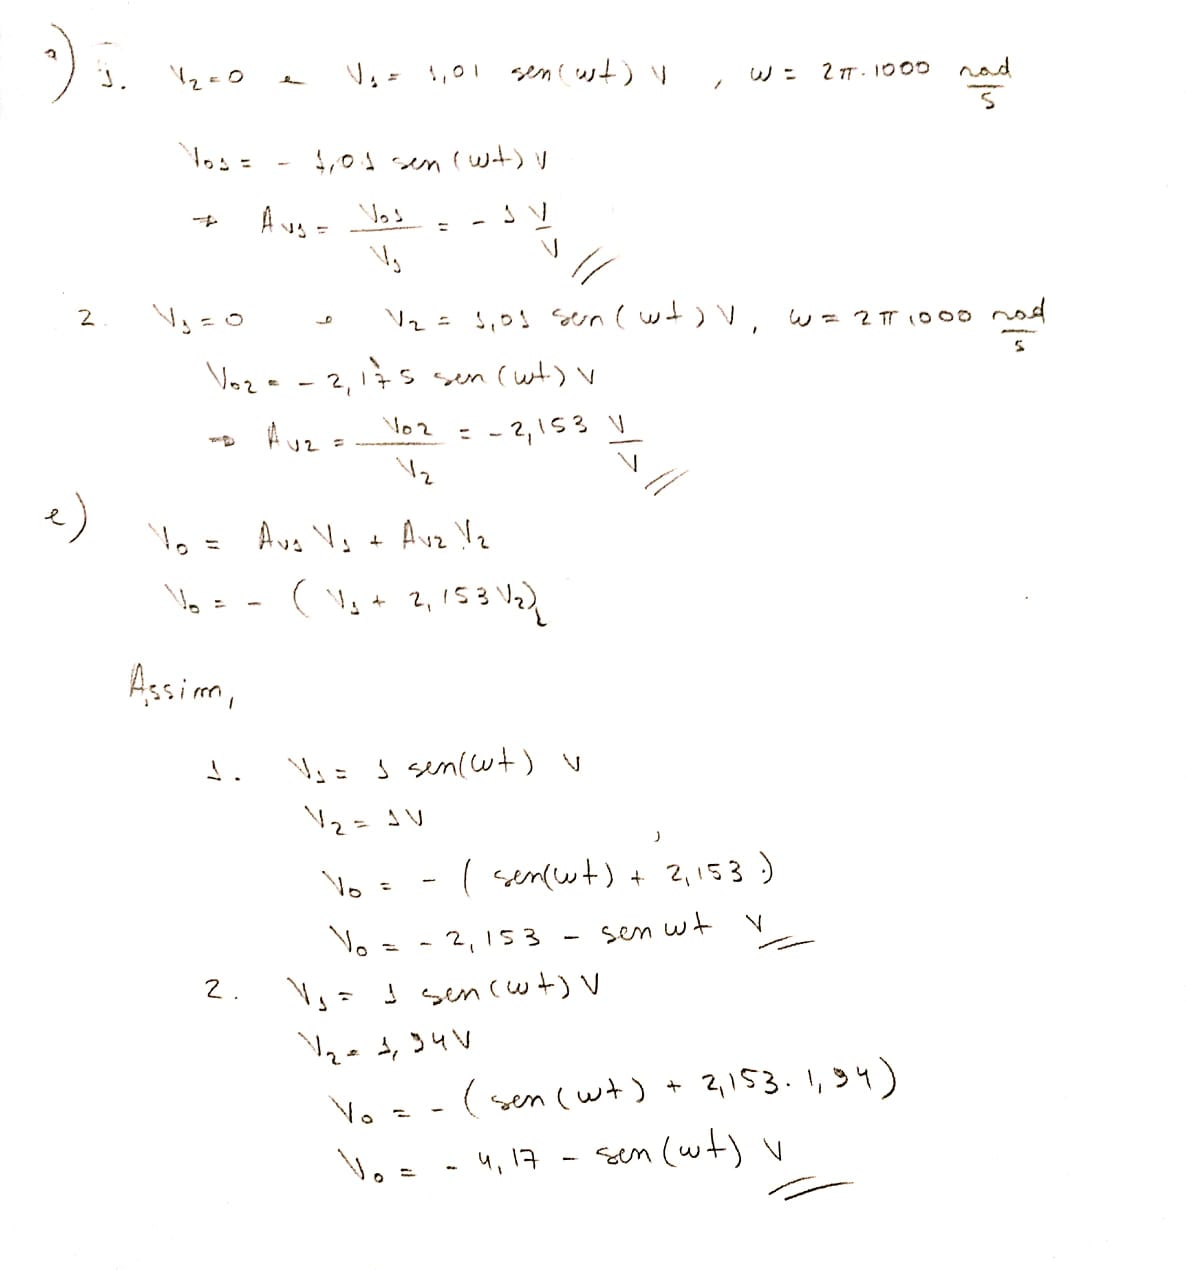
\includegraphics[scale=0.4]{imagens/calc.jpg} 
\centering
\caption{Folha de cálculos da prática.}
\label{p5-2} 
\end{figure} 




     






